
%% bare_jrnl.tex
%% V1.4b
%% 2015/08/26
%% by Michael Shell
%% see http://www.michaelshell.org/
%% fores IEEEtran.cls version 1.8b or later) with an IEEE
%% journar current contact information.
%%
%% This is a skeleton file demonstrating the use of IEEEtran.cls
%% (requil paper.
%%
%% Support sites:
%% http://www.michaelshell.org/tex/ieeetran/
%% http://www.ctan.org/pkg/ieeetran
%% and
%% http://www.ieee.org/

%%*************************************************************************
%% Legal Notice:
%% This code is offered as-is without any warranty either expressed or
%% implied; without even the implied warranty of MERCHANTABILITY or
%% FITNESS FOR A PARTICULAR PURPOSE! 
%% User assumes all risk.
%% In no event shall the IEEE or any contributor to this code be liable for
%% any damages or losses, including, but not limited to, incidental,
%% consequential, or any other damages, resulting from the use or misuse
%% of any information contained here.
%%
%% All comments are the opinions of their respective authors and are not
%% necessarily endorsed by the IEEE.
%%
%% This work is distributed under the LaTeX Project Public License (LPPL)
%% ( http://www.latex-project.org/ ) version 1.3, and may be freely used,
%% distributed and modified. A copy of the LPPL, version 1.3, is included
%% in the base LaTeX documentation of all distributions of LaTeX released
%% 2003/12/01 or later.
%% Retain all contribution notices and credits.
%% ** Modified files should be clearly indicated as such, including  **
%% ** renaming them and changing author support contact information. **
%%*************************************************************************


% *** Authors should verify (and, if needed, correct) their LaTeX system  ***
% *** with the testflow diagnostic prior to trusting their LaTeX platform ***
% *** with production work. The IEEE's font choices and paper sizes can   ***
% *** trigger bugs that do not appear when using other class files.       ***                          ***
% The testflow support page is at:
% http://www.michaelshell.org/tex/testflow/



\documentclass[journal]{IEEEtran}

\usepackage{graphicx}


% correct bad hyphenation here
\hyphenation{op-tical net-works semi-conduc-tor}

\usepackage{graphicx}
\usepackage{caption}

\begin{document}

\title{INF6600 Rapport TP4 \\ Améliorations au système de contrôle d'un drone fermier}


\author{Daniel~Lussier-Lévesque et Ian~Gagnon}

% make the title area
\maketitle

% As a general rule, do not put math, special symbols or citations
% in the abstract or keywords.
\begin{abstract}
L'implémentation d'un système de contrôle de drone fermier a été réalisé progressivement tout au long de la session en commençant par un module TrueTime avec un système continu déjà implémenté en Simulink. Par la suite, l'implémentation a continué sur une machine virtuelle QNX roulant sous VMware, avec certaines fonctions déjà fournies. Ce rapport se concentre sur ce qui a été fait sur cette base de code pour améliorer les aspects les plus importants. La première étape a été d'implémenter un système de log qui nous permettent de voir comment se comporte l'ordonnancement des tâches et la performance du système. Par la suite, malgré le manque de droits d'accès qui nous permettraient de comprendre l'ensemble des problèmes de performances, nous avons toutefois été capable de les mesurer et de les documenter. Un système graphique vivant en dehors de la machine virtuelle nous permettant de valider le comportement du système a aussi été implémenté.
\end{abstract}


\section{Introduction}
\IEEEPARstart{L}{e} système de contrôle considéré est celui d'un drone autonome capable de se déplacer sur trois axes et ayant une caméra fixe pour prendre en photo l'ensemble d'un champs. Le drone doit naviguer les champs et prendre des photos jusqu'à ce que la mémoire soit pleine, puis transmettre les photos à une station base. Lorsque la batterie est presque vide (10\%), le drone doit retourner à la station base pour être rechargé. 

Le système de contrôle implémente le contrôle de la navigation (où le drone va), le contrôle de la batterie (est-il temps d'aller recharger la batterie?) et le contrôle mission (quelle séquence d'étapes doit être exécutés pour opérer avec succès?).

Le système de contrôle de drone sur lequel nous avons apportés nos modifications est un système simple où la communication entre le système continu et discret est effectué par des variables atomiques et par l'enregistrement de \textit{callbacks}. La communication en dehors du système s'effectue par des messages de log sur la console de debug où à intervalle régulier (chaque seconde) l'état du drone est envoyé. Toutes les tâches sont asynchrones les unes par rapport aux autres et roulent sur leur propre fil d'exécution. Nous avons choisi de mettre à jour le système de contrôle du drone toutes les 100 ms.

De plus, l'implémentation du système de contrôle doit être accompagné d'une plateforme de simulation d'un environnement dans lequel opérer, qui comprend le temps de réponse de la caméra, les variations d'orientation et de vitesses, le temps de transmission de photo à la station base et la charge et décharge de la batterie. Le système continu est mis à jour toutes les 20ms de sorte qu'il soit significativement plus rapide que le système de contrôle. De cette manière, le système discret ne voit pas énormément de différence dépendamment s'il se fait juste avant ou juste après une mise-à-jour du système continu.

L'ensemble des photos prises peut être visualisé à travers une carte du monde qui est mis à jour à chaque transmission et montre quelle région a été prise en photo. La carte doit être accédée en allant chercher les fichiers sur le système de fichier de la machine virtuelle.

La politique d'ordonnancement utilisée est un systèmes de priorités fixes et un ordonnancement FIFO pour chaque niveau de priorité. Le choix a été fait de placer la priorité du contrôle caméra avant celle du contrôleur de navigation parce qu'il est plus facile de compenser pour une échéance manquée dans le cas de la navigation (une photo manquée implique de défaire les dernières mise-à-jour de navigation pour reprendre la photo).

La machine virtuelle roule sous QNX 7.0 sous VMware Workstation avec un hôte Windows 10. La machine hôte à un processeur d'Intel à quatre coeurs, le i7 3770, avec 16 GB de mémoire DDR3 et utilise un Seagate ST1000DM003 comme disque dur. 


% An example of a floating figure using the graphicx package.
% Note that \label must occur AFTER (or within) \caption.
% For figures, \caption should occur after the \includegraphics.
% Note that IEEEtran v1.7 and later has special internal code that
% is designed to preserve the operation of \label within \caption
% even when the captionsoff option is in effect. However, because
% of issues like this, it may be the safest practice to put all your
% \label just after \caption rather than within \caption{}.
%
% Reminder: the "draftcls" or "draftclsnofoot", not "draft", class
% option should be used if it is desired that the figures are to be
% displayed while in draft mode.
%
%\begin{figure}[!t]
%\centering
%\includegraphics[width=2.5in]{myfigure}
% where an .eps filename suffix will be assumed under latex, 
% and a .pdf suffix will be assumed for pdflatex; or what has been declared
% via \DeclareGraphicsExtensions.
%\caption{Simulation results for the network.}
%\label{fig_sim}
%\end{figure}

% Note that the IEEE typically puts floats only at the top, even when this
% results in a large percentage of a column being occupied by floats.


% An example of a double column floating figure using two subfigures.
% (The subfig.sty package must be loaded for this to work.)
% The subfigure \label commands are set within each subfloat command,
% and the \label for the overall figure must come after \caption.
% \hfil is used as a separator to get equal spacing.
% Watch out that the combined width of all the subfigures on a 
% line do not exceed the text width or a line break will occur.
%
%\begin{figure*}[!t]
%\centering
%\subfloat[Case I]{\includegraphics[width=2.5in]{box}%
%\label{fig_first_case}}
%\hfil
%\subfloat[Case II]{\includegraphics[width=2.5in]{box}%
%\label{fig_second_case}}
%\caption{Simulation results for the network.}
%\label{fig_sim}
%\end{figure*}


\section{Lacunes du système de base}
\label{lacunes}

Le système décrit plus haut a plusieurs lacunes importantes. Nous allons ici nous focaliser sur les trois principales faiblesses qui nous ont empêcher de réaliser correctement plusieurs améliorations auxquels nous avions pensés. Il va s'en dire que nous avons penser plus important de régler ces lacunes au meilleur de nos capacités en priorité.

\subsection{Peu de visibilité sur l'état du système}

Le principal problème est qu'avec le système de base, nous ne savons pas si le système est \emph{correct}, c'est à dire que le système effectue les actions que l'ont s'attend à ce qu'il fasse. Les messages de logs qui sont envoyés sont répétitifs et il est facile de manquer un comportement anormal dans les 1800 messages que comportent une séquence d'exécution. De plus, il est impossible de savoir ce qui se passe à l'intérieur de cette période d'une seconde. une période plus courte n'est toutefois pas envisageable: il serait impossible d'analyser l'entièreté du message en temps réel et donc encore plus facile de manquer une information inattendue. Il n'est pas non plus envisageable d'analyser les données à la fin de la simulation: la console de debug ne peut contenir qu'un nombre limité de messages.

En conséquence, il n'est pas possible de qualifier le système d'aucune manière: un problème de comportement du système demanderait une correction importante au code qui invaliderait l'ensemble des mesures effectués. Comme une séance de simulation dure 30 minutes, il serait difficile d'arriver à un ensemble de résultat suffisant dans un temps raisonnables si nos mesures devaient être invalidés. Sans mesures fiables, il est impossible de déterminer si une tentative d'amélioration du système améliore réellement le système. Pour cette raison, cette lacune est considérée comme la plus importante du système implémenté.

\subsection{Aucune visibilité sur la qualité de l'ordonnancement}

En assumant que le comportement du système est correct, nous ne pouvons toujours pas penser à améliorer les performances du système ou rajouter de nouvelles fonctions utiles parce que nous n'avons aucune métrique de performance de disponible. Nous ne savons pas si les tâches manquent leur échéance de manière régulière et arrivent tout juste à rester fonctionnels, ou au contraire si il y a largement de ressources disponibles pour de nouvelles tâches.

Dans le cas où le comportement du système n'est pas celui attendu, les métriques de qualité d'exécution nous sont aussi utile pour comprendre les problèmes. Si une tâche est en famine parce que les tâches plus prioritaires prennent toutes les ressources, ce sera facilement visible et évitera une longue séance de debug en aveugle. Nous considérons cette lacune comme fondamentale et bloquante pour des améliorations à d'autres aspect du système.

\subsection{Pics de latence}

Après avoir apportés les modifications qui seront détaillés à la section \ref{ameliorations}, nous avons réalisés que le système tel que simulé avait encore une lacune qui bloquait des améliorations que nous avions planifiés: le système est affecté par des pics de latences non-déterministes. Ces pics de latences affectent toutes les tâches en même temps. Plus spécifiquement, ils affectent des tâches qui n'acquirent pas de mutex où autre verrou global et communiquent uniquement par des variables atomiques. On peut donc conclure que ces pics arrivent au niveau système et non au niveau de l'ordonnancement ou au niveau de la communication. 

En plus d'affecter les performances du systèmes et de le rendre moins fiable, un impact important de ces pics de latences est que toutes les métriques de pire temps d'exécution ou de déviations standard sont affectés de manière aléatoire et qu'une comparaison avant et après d'une tentative d'amélioration est noyée dans le bruit de ces pics.

Les pics des latences durent plusieurs millisecondes. Plusieurs tentatives de contourner le problème ont été essayé: réduire le nombre de cœurs du système de contrôle, augmenter le nombre de cœurs du système et déplacer la machine virtuelle du disque réseau au disque dur local. Déplacer la machine virtuelle à permis de réduire significativement la durée de ces pics, mais aucune des ces tentatives n'a permis de ramener les variations de latences à des temps raisonnables.

\section{Améliorations apportées}
\label{ameliorations}
\begin{figure}
	\centering
	\captionsetup{justification=centering}
	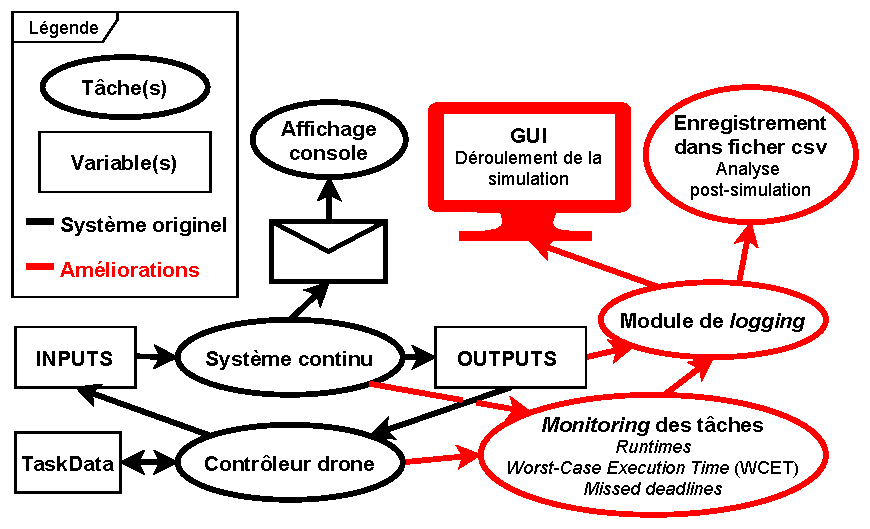
\includegraphics[width=3.5in]{diagrammeDeTaches_Simple.pdf}
	\caption{Diagramme de tâches du système}
	\label{taskDiagram}
\end{figure}

\begin{figure}
  
\includegraphics[width=\linewidth]{placeholder.png}
  \caption{Diagramme des améliorations apportés}
  \label{fig:ameliorations}
\end{figure}

Comme il est possible de le voir à la figure \ref{fig:ameliorations}, les améliorations ont été apportés au niveau du \textit{logging} et du \textit{monitoring} des tâches pour avoir des sorties de simulations faciles à interpréter et qui corrigent les deux premières lacunes décrites à la section \ref{lacunes}, le manque de lisibilité de ce qui se passe dans le système.

\subsection{Monitoring des tâches}

Pour chaque tâche qui s'exécute, une mesure du temps d'une exécution est faite à l'aide de \verb|std::chrono::steady_clock::now()|. Deux variables (atomiques) sauvegarde la valeur de la dernière exécution et le pire cas. Dans le cas de notre système, nous n'avons pas d'horloge permettant une granularité plus grande qu'une milliseconde.

\subsection{Logging}

Une fois que nous avons implanté le code pour avoir l'information dans des variables, il faut penser à un moyen de la communiquer. Il a donc fallu implémenter une nouvelle fonction (avec le code de \textit{monitoring} associé) pour lire l'ensemble des variable et les pousser vers les nouvelles sorties. Nous avons décider d'exécuter la tâche toutes les 100 millisecondes afin de ne pas surcharger le système. Cette fonction est appelée par la tâche de \textit{monitoring} déjà existante qui auparavant ne poussait les donnée que vers la console une fois toute les secondes.

\subsection{Sortie en fichier csv}

La sortie qui permet de faire une analyse compréhensive du système est un simple fichier csv qui est sauvegardé en mémoire non-volatile au fur et à mesure que la simulation avance (de sorte qu'un \textit{crash} peut être investigué en s'aidant du fichier). Le format csv étant supporté par pratiquement tous les outils d'analyse et de base de données, il est facile de s'en servir pour obtenir des statisques sur un grand nombre d'exécutions, de réaliser des analyses et des graphiques en Python, en R, en MATLAB ou tout simplement dans Microsoft Excel ou LibreOffice Calc.

\subsection{GUI}

\#TODO

\begin{figure}
  
\includegraphics[width=\linewidth]{placeholder.png}
  \caption{Le gui en action}
  \label{fig:GUI}
\end{figure}

\section{Résultats}


\section{Conclusion}
The conclusion goes here.



% if have a single appendix:
%\appendix[Proof of the Zonklar Equations]
% or
%\appendix  % for no appendix heading
% do not use \section anymore after \appendix, only \section*
% is possibly needed

% use appendices with more than one appendix
% then use \section to start each appendix
% you must declare a \section before using any
% \subsection or using \label (\appendices by itself
% starts a section numbered zero.)
%

% references section

% can use a bibliography generated by BibTeX as a .bbl file
% BibTeX documentation can be easily obtained at:
% http://mirror.ctan.org/biblio/bibtex/contrib/doc/
% The IEEEtran BibTeX style support page is at:
% http://www.michaelshell.org/tex/ieeetran/bibtex/
%\bibliographystyle{IEEEtran}
% argument is your BibTeX string definitions and bibliography database(s)
%\bibliography{IEEEabrv,../bib/paper}
%
% <OR> manually copy in the resultant .bbl file
% set second argument of \begin to the number of references
% (used to reserve space for the reference number labels box)
\begin{thebibliography}{1}

\bibitem{IEEEhowto:kopka}
H.~Kopka and P.~W. Daly, \emph{A Guide to \LaTeX}, 3rd~ed.\hskip 1em plus
  0.5em minus 0.4em\relax Harlow, England: Addison-Wesley, 1999.

\end{thebibliography}




% Can be used to pull up biographies so that the bottom of the last one
% is flush with the other column.
%\enlargethispage{-5in}



% that's all folks
\end{document}


